\documentclass[11pt]{article}
% Horizontal Magnetic Dipole over a lossy half-space
\usepackage[utf8]{inputenc} % Use it to include other characters than ABC
\usepackage[cmex10]{amsmath}
\usepackage{mdwmath}
\usepackage{mdwtab}
\usepackage{hyperref}
\usepackage{physics} % For using the oridnary derivative nomenclature
\usepackage{datetime} % Insert date and time
\usepackage[letterpaper, margin=1in]{geometry}
\usepackage{graphicx}
\usepackage{pgfplots}
\usepackage{tikz}
\usepackage{standalone}
\usepackage[americanresistors,americaninductors]{circuitikz}
\usetikzlibrary{positioning}
\usetikzlibrary{arrows}
\usepackage{subfig}
\usepackage{mathptmx} % Times new Roman

% ------------------------------- Useful Tricks Learnt
% Use ={}& to align subequations to the left
% Use = for single equations
% Put comments % in between the lines in order to avoid forming a new paragraph.
% To enter special characters into Inkspace figures, use Ctrl+U and then enter       the unicode. e.g., for \times symbol, the unicode is U+0D7. So the key entry would be Ctrl+U U+0d7 and then press enter.
%
% ----------------- To compile with references use the following order in Shell"
% 1. pdflatex filename.tex
% 2. bibtex filename (no extension)
% 3. bibtex filename (no extension)
% 4. pdflatex filename.tex
% -----------------

% Personal definitions
% Operators
\renewcommand{\v}[1]{\mathbf{#1}} % vectors
\newcommand{\ti}[1]{\tilde{#1}} % spectral representation

% Symbols
\renewcommand{\O}{\omega}  % omega
\newcommand{\E}{\varepsilon}  % epsilon
\renewcommand{\u}{\mu}  % mu
\newcommand{\p}{\rho}  % rho
\newcommand{\x}{\times}  % times
\renewcommand{\inf}{\infty}  % infinity
\newcommand{\infint}{\int\limits_{-\inf}^\inf} % integral by R
\newcommand{\del}{\nabla}  % nabla operator
\renewcommand{\^}{\hat}  % unit vector
\newcommand*\diff{\mathop{}\!\mathrm{d}} % Define differential operator

\definecolor{s1}{RGB}{204, 76, 2}

\begin{document}
  \title{\textsc{Numerical Integration of Sommerfeld Integrals}\\}
  \date{\footnote{Last Modified: \currenttime, \today.}}
  \maketitle

  The fields of sources in a layered media environment involves computation of Sommerfeld Integrals which are reminiscent of a Hankel transform (a Fourier transform in cylindrical coordinate system):

  \begin{equation}
    \int_{0}^{\inf} \ti{G}(k_{\p}; \v{r}|\v{r}') J_n(k_{\p} \p) k_{\p} \diff{k_{\p}}
    \label{eq:SI}
  \end{equation}

  where $\ti{G}$ is a spectral domain Green's function of the structure, $\v{r}$ and $\v{r}'$ are the observation and source locations respectively, and $J_n$ is bessel's function of order $n$. In most cases, integral in (\ref{eq:SI}) cannot be solved analytically. Furthermore, due to singularities and oscillations in the integrand, the numerical evaluation  requires careful manipulation and techniques. Using the Cauchy's Integral Theoerem \cite[p. 377]{arfken2001mathematical} by selecting the path of integration along the positive real axis in the complex $k_{\p}$ plane as shown in Fig. \ref{fig:path}. \cite{golubovic2012efficient,michalski2016efficient}.

  \begin{figure}[h!]
    \centering
    \includestandalone[width=1\textwidth]{figures/path}
    \caption{Integration Path along the real axis}
    \label{fig:path}
  \end{figure}

The integral in (\ref{eq:SI}) is computed by splitting into three sections:

\begin{equation}
  \int_{0}^{\inf} \ti{G}(k_{\p}; \v{r}|\v{r}') J_n(k_{\p} \p) k_{\p} \diff{k_{\p}} = \left(\int_{0}^{\gamma} + \int_{\gamma}^{a} + \int_{a}^{\inf} \right)
  \ti{G}(k_{\p}; \v{r}|\v{r}') J_n(k_{\p} \p) k_{\p} \diff{k_{\p}}
  \label{eq:SI_split}
\end{equation}

where $\gamma$ represents a slight detour of the integration path from the real axis. This is done to bypass the singularity lying on the real axis. The real part of $\gamma$ is the same as the singularity location, $k$ whereas the imaginary part should be as small as possible to avoid wild growth of the bessel function illustrated in Fig. \ref{fig:bessel}. Furthermore, $a$ represents a breakpoint, where we switch the numerical integration routine.

\begin{figure}[h!]
  \centering
  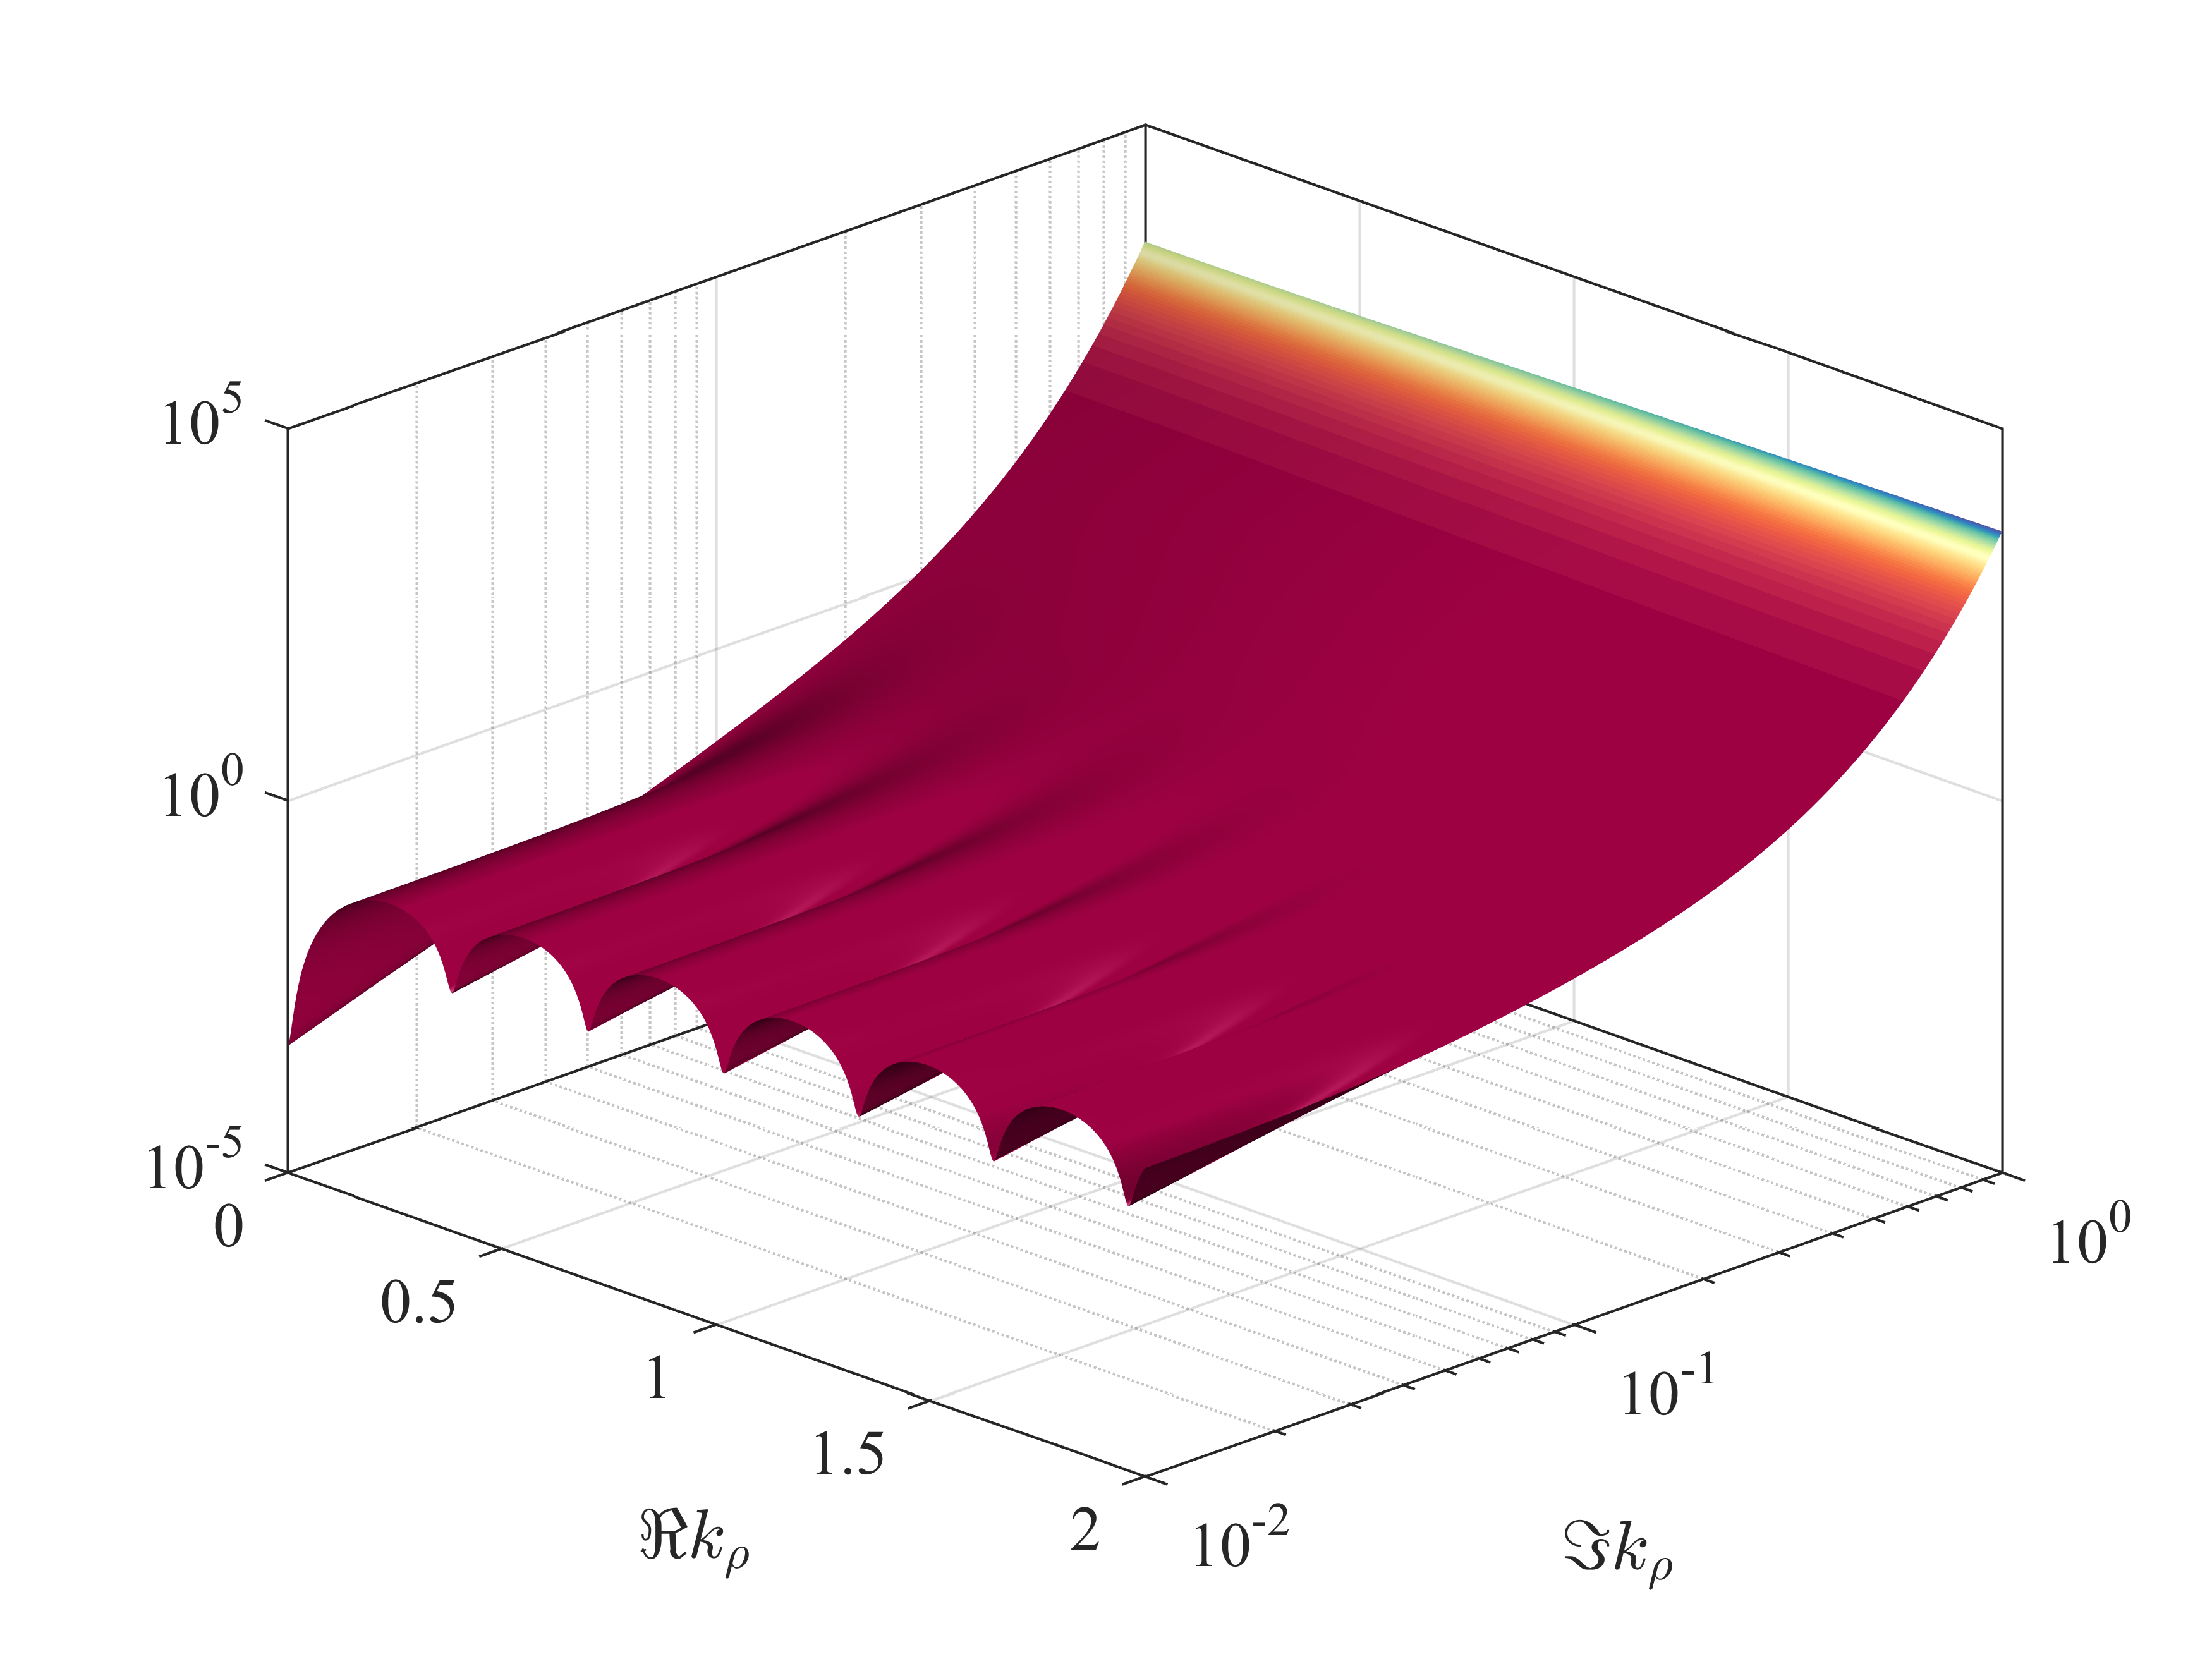
\includegraphics[width=\textwidth]{figures/J_1_comp.png}
  \caption{Exponential Growth of Bessel function $J_1(10 k_{\p})$ along the imaginary axis}
  \label{fig:bessel}
\end{figure}

\section{Overview of Numerical Integration}




  \clearpage % Force Bibliography to the end of document
  \bibliography{refs}
  \bibliographystyle{ieeetr}

\end{document}
